\documentclass{article}[a4paper]

\usepackage[czech]{babel}
\usepackage[T1]{fontenc}
\usepackage{geometry}
\usepackage{graphicx}
\usepackage[pdfusetitle]{hyperref}

\title{Implementační dokumentace k~1. úloze do IPP 2023/2024}
\author{Milan Vodák}

\begin{document}
    \begin{center}
        {\Large Implementační dokumentace k~1. úloze do IPP 2023/2024}

        Jméno a příjmení: Milan Vodák

        Login: xvodak07
    \end{center}

    \section{Diagram tříd}

    \begin{center}
        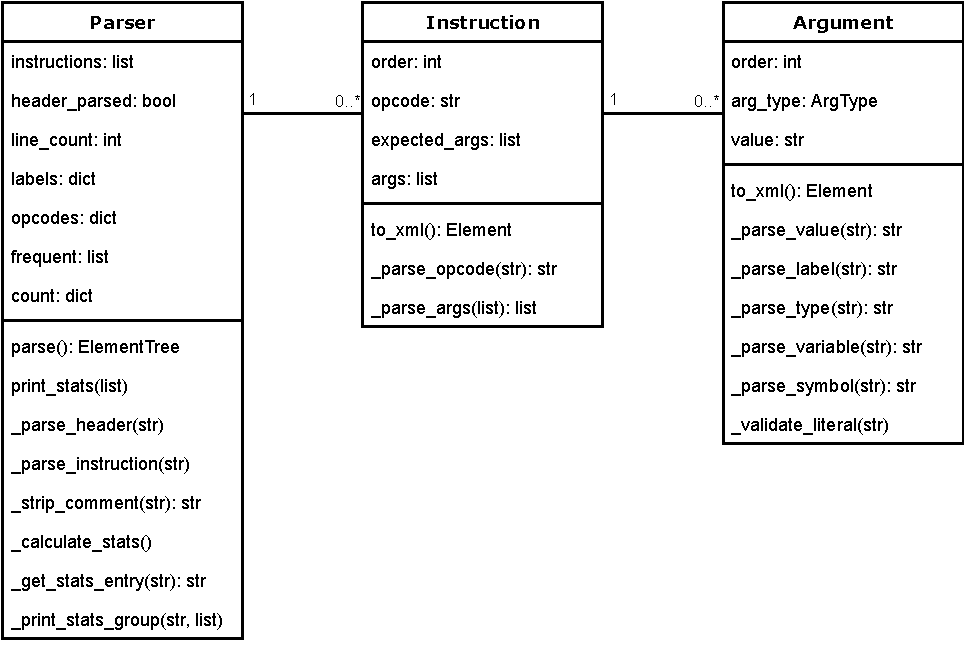
\includegraphics[width=0.95\textwidth]{class-diagram.pdf}
    \end{center}

    \section{Popis částí}

    \subsection{\texttt{Parser}}

    Třída \texttt{Parser} reprezentuje samotný syntaktický analyzátor.
    Většinu analyzační logiky zastřešuje metoda \texttt{parse()}, která čte řádek po řádku ze standardního vstupu a zpracovává je.
    Jako první z~řádku prostřednictvím metody \texttt{\_strip\_comment()} odstraní komentáře a také přebytečné bílé znaky a následně řádek zpracuje jako hlavičku, nebyla-li tato nalezena; nebo jako instrukci.
    Prázdné řádky či řádky obsahující pouze komentář jsou ignorovány.
    Dostane-li se analyzátor na konec standardního vstupu zatímco stále nenašel hlavičku, ukončí program s~návratovým kódem 23.

    O~zpracování hlavičky a instrukce se starají pomocné metody analyzátoru \texttt{\_parse\_header()}, resp. \texttt{\_parse\_instruction()}.
    Po nalezení správné hlavičky je nastaven příznak \texttt{header\_parsed} a na další řádky už je nahlíženo jen jako na instrukce.
    Zpracování instrukce je delegováno na třídu \texttt{Instruction} (viz Sekce \ref{sec:instruction}) a získaná instance se vloží
    do seznamu doposud načtených instrukcí, tj. instančního atributu \texttt{instructions}.
    V~této fázi se analyzátor také stará o~ošetření výjimek, jež mohou být vyvolány během konstrukce instrukcí a jejich argumentů.
    To spočívá ve výpisu hlášky s~číslem dotčeného řádku na standardní chybový výstup a v~ukončení programu s~odpovídajícím návratovým kódem.

    Pro generování výstupní XML reprezentace jsem použil knihovnu \texttt{xml.etree.ElementTree}.
    Po zpracování celého standardního vstupu se vytvoří kořenový element \texttt{<program>} a iterativně se instrukce ze seznamu \texttt{instructions}
    převádějí na XML elementy, které jsou dovnitř kořenového elementu vkládány.
    Nakonec metoda \texttt{parse()} vrátí XML strom zpracovaného programu.

    \subsection{\texttt{Instruction}}
    \label{sec:instruction}

    Instance třídy \texttt{Instruction} odpovídá jedné instrukci vstupního programu a uchovává v~sobě pořadí instrukce, operační kód, očekávané typy argumentů a seznam skutečně načtených argumentů.
    Konstruktor třídy předá postupně kontrolu pomocným metodám \texttt{\_parse\_opcode()} a \texttt{\_parse\_args()}.
    Hotovou instrukci je možné převést na XML element voláním metody \texttt{to\_xml()}.

    Instrukční sada je reprezentována slovníkem \texttt{INSTRUCTION\_SET}, jehož záznamy se skládají z~operačního kódu jako klíče a ze seznamu typů argumentů, které instrukce očekává.

    Po validaci obdrženého operačního kódu za použití regulárního výrazu\footnote{Výskyt jiného znaku než velkých či malých písmen na místě, kde se očekává operační kód, je považován za syntaktickou chybu,
    která vede na ukončení programu s~návratovým kódem 23. Neúspěšné vyhledání operačního kódu v~instrukční sadě vyvolá výjimku \texttt{InvalidOpcodeError}.}
    je z~instrukční sady vybrán záznam odpovídající instrukce a následně je instanci nastaven operační kód (velkými písmeny) a očekávané typy argumentů.
    Na základě těchto typů se následně provádí konstrukce argumentů ze slov načtených za operačním kódem (viz Sekce \ref{sec:argument}) a ty jsou přidávány do seznamu \texttt{args}.

    \subsection{\texttt{Argument}}
    \label{sec:argument}

    Argument sestává z~jeho pořadí v~rámci instrukce, typu vyjádřeného výčtovým typem \texttt{ArgType} a hodnoty, která bude vypsána do výstupního XML.
    Obdobně jako u~instrukce, převod na XML reprezentaci zajišťuje metoda \texttt{to\_xml()}.
    Konstruktor třídy \texttt{Argument} požaduje na vstupu typ argumentu, který je očekáván, a na základě tohoto typu je provedeno ověření správnosti načtené hodnoty a případně její úprava do výstupního formátu.

    Očekává-li se návěští, typ, nebo proměnná, validace probíhá jednoduše pomocí regulárních výrazů.
    V~případě symbolu může být argument buď proměnná nebo konstanta, což se rozhoduje podle části identifikátoru před znakem \texttt{@} a následně je patřičně upřesněn typ atributu.
    Jedná-li se o~konstantu, metoda \texttt{\_validate\_literal()} regulárními výrazy ověří správnost druhé části zápisu.
    V~případě nesprávně zapsaného argumentu či výskytu argumentu neočekávaného typu se vyvolá výjimka \texttt{ParserError} s~konkrétní chybovou zprávou.

    \section{Rozšíření \texttt{STATP}}

    Implementoval jsem rozšíření umožňující výpis statistik o vstupním programu.
    Argumenty příkazové řádky jsou načteny a zvalidovány funkcí \texttt{parse\_input\_args()}.
    Jsou-li přítomné argumenty týkající se statistik, zavolá se metoda \texttt{print\_stats()} třídy \texttt{Parser},
    která nejprve prostřednictvím metody \texttt{\_calculate\_stats()} spočítá projitím seznamu instrukcí všechna statistická data,
    a následně zpracuje vyžádané skupiny statistik, které nakonec postupným voláním metody \texttt{\_print\_stats\_group()} vypíše do souborů.
    Chyba v argumentech je indikována vyvoláním výjimky \texttt{OptionsError}.
\end{document}
